\documentclass[border=2pt]{standalone}
\usepackage{pgfplots}
\pgfplotsset{compat=1.18}
\begin{document}
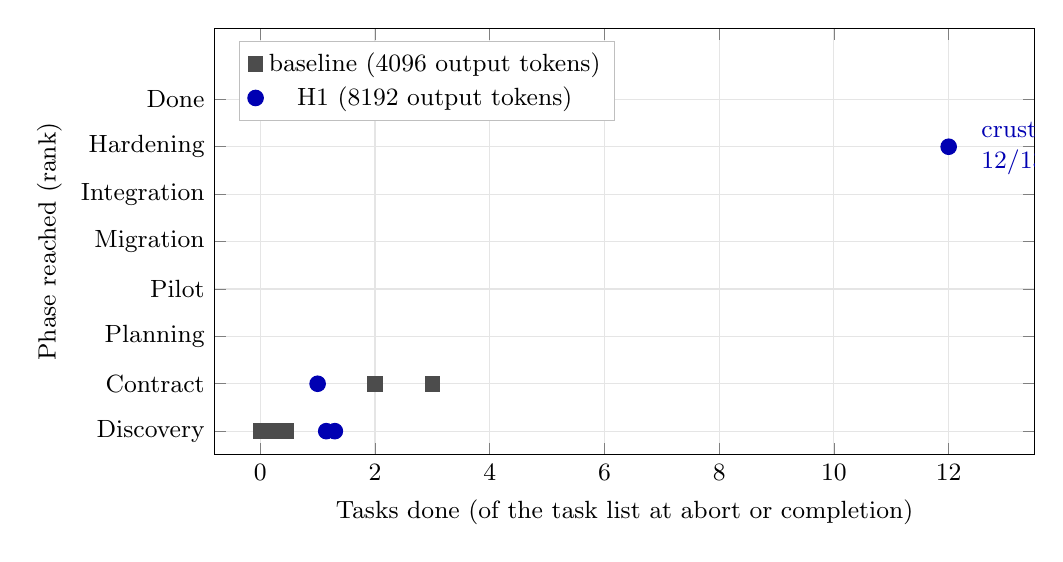
\begin{tikzpicture}
\begin{axis}[
  width=12cm,
  height=7cm,
  xlabel={Tasks done (of the task list at abort or completion)},
  ylabel={Phase reached (rank)},
  ymin=-0.5, ymax=8.5,
  xmin=-0.8, xmax=13.5,
  ytick={0,1,2,3,4,5,6,7},
  yticklabels={Discovery, Contract, Planning, Pilot, Migration, Integration, Hardening, Done},
  grid=major,
  grid style={gray!20},
  legend style={at={(0.03,0.97)}, anchor=north west, font=\small, draw=gray!50},
  tick label style={font=\small},
  label style={font=\small},
]
% Cycle-1 autooptimise per problem set, from .artifacts/experiments/SUMMARY.md.
% Phase rank: Discovery=0, Contract=1, Hardening=6. Rows with "no data"
% (daemon death) carry no phase or task data; the caption scores them as
% zero. Baseline rows: colorsys 3/6 Contract, nandc relaunch 2/5 Contract,
% utf8 0/2, libm17 relaunch 0/3, oxidizer 0/3, alphatrans relaunch 0/3
% (all Discovery). H1 rows with data: nandc 12/13 Hardening, utf8 1/5
% Contract, oxidizer 1/5 Discovery, alphatrans 0/1 Discovery.
% Overlapping Discovery points are jittered horizontally so each run
% stays visible.
\addplot[
  only marks, mark=square*, mark size=2.6pt, color=gray!60!black,
] table {
x y
3 1
2 1
0 0
0.15 0
0.3 0
0.45 0
};
\addlegendentry{baseline (4096 output tokens)}

\addplot[
  only marks, mark=*, mark size=2.8pt, color=blue!70!black,
] table {
x y
12 6
1 1
1.15 0
1.3 0
};
\addlegendentry{H1 (8192 output tokens)}

% Champion annotation: the only candidate that produced a translated,
% toolchain-verified project.
\node[font=\small, text=blue!70!black, anchor=west, align=left]
  at (axis cs:12.4,6) {crust/nandc: Hardening,\\12/13 tasks, 2/2 tests pass};

\end{axis}
\end{tikzpicture}
\end{document}
